\section{Ejercicio 4}

Considere la misma señal de mensaje y portadora del Ejercicio 2, pero utilice un modulador producto.

\begin{enumerate}[label=\alph*)]
    \item Expresar analíticamente $s(t)$ y $S(f)$. Graficar resultados y explicar cuál fue el cambio en la señal de salida del modulador.
    \item Considerando que la señal de salida del modulador se aplica a un detector coherente (ver Fig. 2), y que las portadoras tanto en el transmisor como en el receptor se encuentran en perfecto sincronismo: obtener $v(t)$ y graficar su espectro.
    \item Ahora suponer que hay una diferencia de fase entre portadoras. Comentar por qué esto es importante y qué sucede en casos extremos.
\end{enumerate}

\begin{figure}[h!]
    \centering
    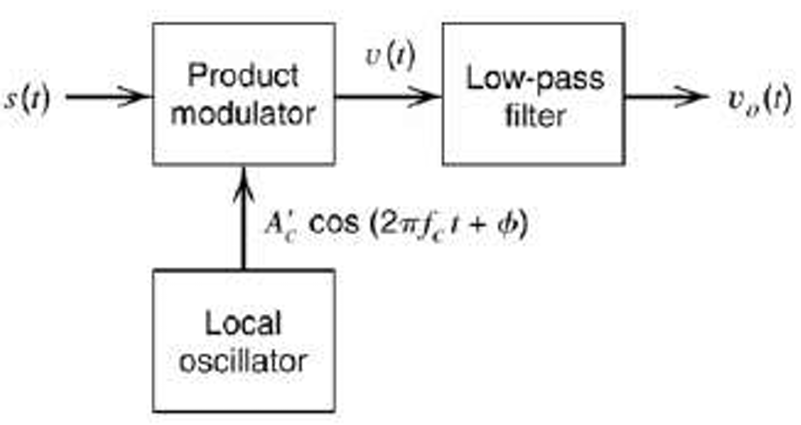
\includegraphics[width=0.7\textwidth]{imagenes/Parte_1/Actividad_4/fig2.png}
    \caption{Detector coherente}
\end{figure}
